\documentclass[a4j,twocolumn]{jarticle}
\usepackage[utf8]{inputenc}
\usepackage[cmex10]{amsmath}
\usepackage{amssymb,verbatim}
\usepackage[dvipdfmx]{graphicx}
\usepackage{mathrsfs}
\usepackage{here}
\usepackage{tabularx}

\usepackage{geometry}
\geometry{left=20mm,right=20mm,top=20mm,bottom=20mm}
\fontsize{14pt}{10pt}\selectfont
\def \figref #1{\figurename\ref{#1}}
\def \tbref #1{\tablename\ref{#1}}
\def \equref #1{式(\ref{#1})}
%\vspace{-20cm}
\title{\vspace{-2em}B06 Y00-量子暗号における増幅の効果\\
\vspace{0.5cm}
\normalsize{Effect of Amplification for Y00 Quantum Cipher}}
\date{}
\pagestyle{empty}
\author{量子情報数理研究室\hspace{50mm}酒寄 遥}
\begin{document}
\maketitle
\thispagestyle{empty}
\section{はじめに}
本論文では,減衰通信路におけるY00-量子暗号のシミュレーションシステムを用いて,正規受信者の誤り率を評価する.特に増幅器を設置したときの効果について考察する.
\section{Y00-量子暗号の信号状態}
まず,コヒーレント状態について説明する.コヒーレント状態は,複素振幅$\alpha=x+iy$を持つ理想的なレーザー光を表す量子状態である.コヒーレント状態の複素振幅$\alpha$は複素平面上で平均$(x,y)^T$,共分散行列 
\begin{equation}\label{eq1}
\begin{pmatrix}
1/4&0\\
0&1/4
\end{pmatrix}
\end{equation}
の正規分布に従って揺らいでいる.
\figref{Fig:3_1}は,平均$(0,0)^T$のコヒーレント状態の揺らぎを表している.

\begin{figure}[htbp]
        \centering   
        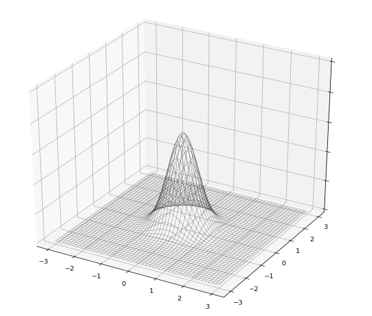
\includegraphics[width=0.4\textwidth]{img/zemi33.png}
        \caption[sample image (png)]{コヒーレント状態のゆらぎ}
        \label{Fig:3_1}
    \end{figure}
図\ref{Fig:3_2}
を用いて
Y00-量子暗号の信号状態について説明する.図\ref{Fig:3_2}において白丸がコヒーレント状態を表している.Y00-量子暗号状態では使用する基底によって0と1に対応する信号状態が異なる.例えば基底1を使って0を送りたいときはXのコヒーレント状態を使い,1を送りたいときはYのコヒーレント状態を使う.正規の受信者と送信者は通信に使用する基底の情報を共有している.これに対し盗聴者は基底の情報を持っておらず,盗聴が非常に困難となるため,安全性が保証される.$S_{max}$は信号の最大強度を表している.$B$個の基底で通信する場合隣接信号間の間隔は$S_{max}/2B-1$になる.このことより基底$k$の信号状態は

$$
\left |\frac{S_{max}}{2B-1}\right\rangle,\left |\frac{S_{max}}{2B-1}(B+k)\right\rangle
$$
で与えられる.
\begin{figure}[htbp]
        \centering   
        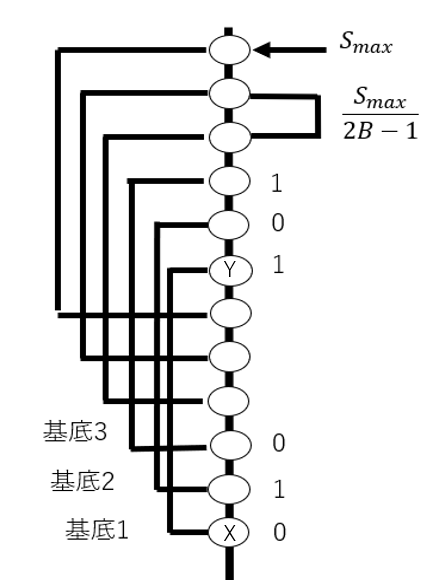
\includegraphics[width=0.2\textwidth]{img/zemi30.png}
        \caption[sample image (png)]{量子暗号の信号状態.}
        \label{Fig:3_2}
    \end{figure}
    
\section{Y00-量子暗号システム}
Y00-量子暗号のシステムについて説明する.送信者と受信者はseedkeyを共有している.まず線形フィードバックシフトレジスタ(LFSR)によって疑似乱数を発生させる.
このとき,seedkeyが同じであるので発生する乱数も同じとなる.乱数は基底番号を表し,送信者と受信者は同じ基底番号を使うことができる.送信器では送信バイナリデータと基底番号の値に対応する量子状態を送信する.受信器では受け取った量子状態と基底番号を使ってバイナリデータを出力する.次に受信器における処理について説明する.

\begin{figure}[htbp]
        \centering   
        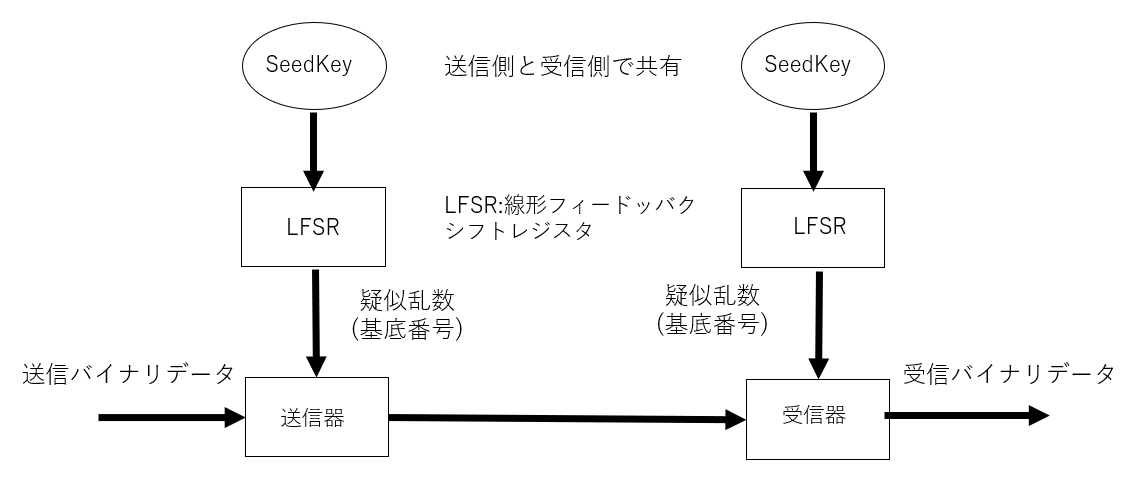
\includegraphics[width=0.4\textwidth]{img/zemi1-1-2.png}
        \caption[sample image (png)]{量子暗号システム.}
        \label{fig:4_1}
    \end{figure}



受信器ではまずホモダイン測定を行う.ホモダイン測定はコヒーレント状態の複素振幅$\alpha=x+iy$の$x$成分を測定する.
\begin{figure}[htbp]
        \centering   
        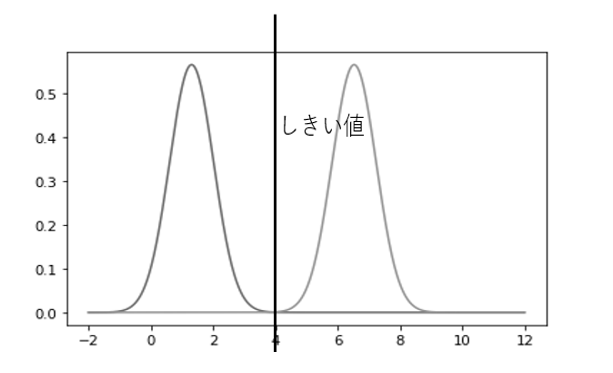
\includegraphics[width=0.4\textwidth]{img/zemi31.png}
        \caption[sample image (png)]{をホモダイン測定時の
出力の確率分布.}
        \label{fig:4_2}
    \end{figure}
コヒーレント状態をホモダイン測定した場合の出力の確率分布は,図\ref{fig:4_2}のように,分散$1/4$の正規分布になっている.受信器では,測定値に基づき,しきい値を使って受信したデータが0か1か判断する.すなわち,基底番号が奇数の場合,測定値がしきい値より大きければ1,小さければ0と判定する.一方基底番号が偶数の場合,測定値がしきい値より大きければ0,小さければ1と判定する.

\section{減衰と増幅}
今回の評価実験では通信路が減衰の影響を受ける場合について考える.
透過率$k$の減衰を受けることにより,平均$\mu$は$\sqrt{k}\mu$となる.
また,共分散行列$A$は,$kA+ (1-k)I_2/4$となる.ここで,$I_2$は$2\times 2$の単位行列を表す.
一方,増幅率$G>1$で増幅すると平均$\mu$は$\sqrt{G}\mu$となり,共分散$A$は,$GA+(G-1)I_2/4$となる.


\section{評価実験}


\figref{Fig:5_4}は信号の最大強度が5,基底数が256,送信データ数が1000個の場合に透過率と正規受信者の誤り率の関係を表したもので,横軸は透過率,縦軸は誤り率となっている.グラフからわかる通り,信号の減衰に合わせてしきい値調整することで,透過率が$k<0.6$のときに誤り率を大幅に減らすことができることがわかる.一方透過率が$0.8<k$のときはしきい値調整をしなくても信号の誤り率が低くなることがわかる.

  
\begin{figure}[htbp]
        \centering   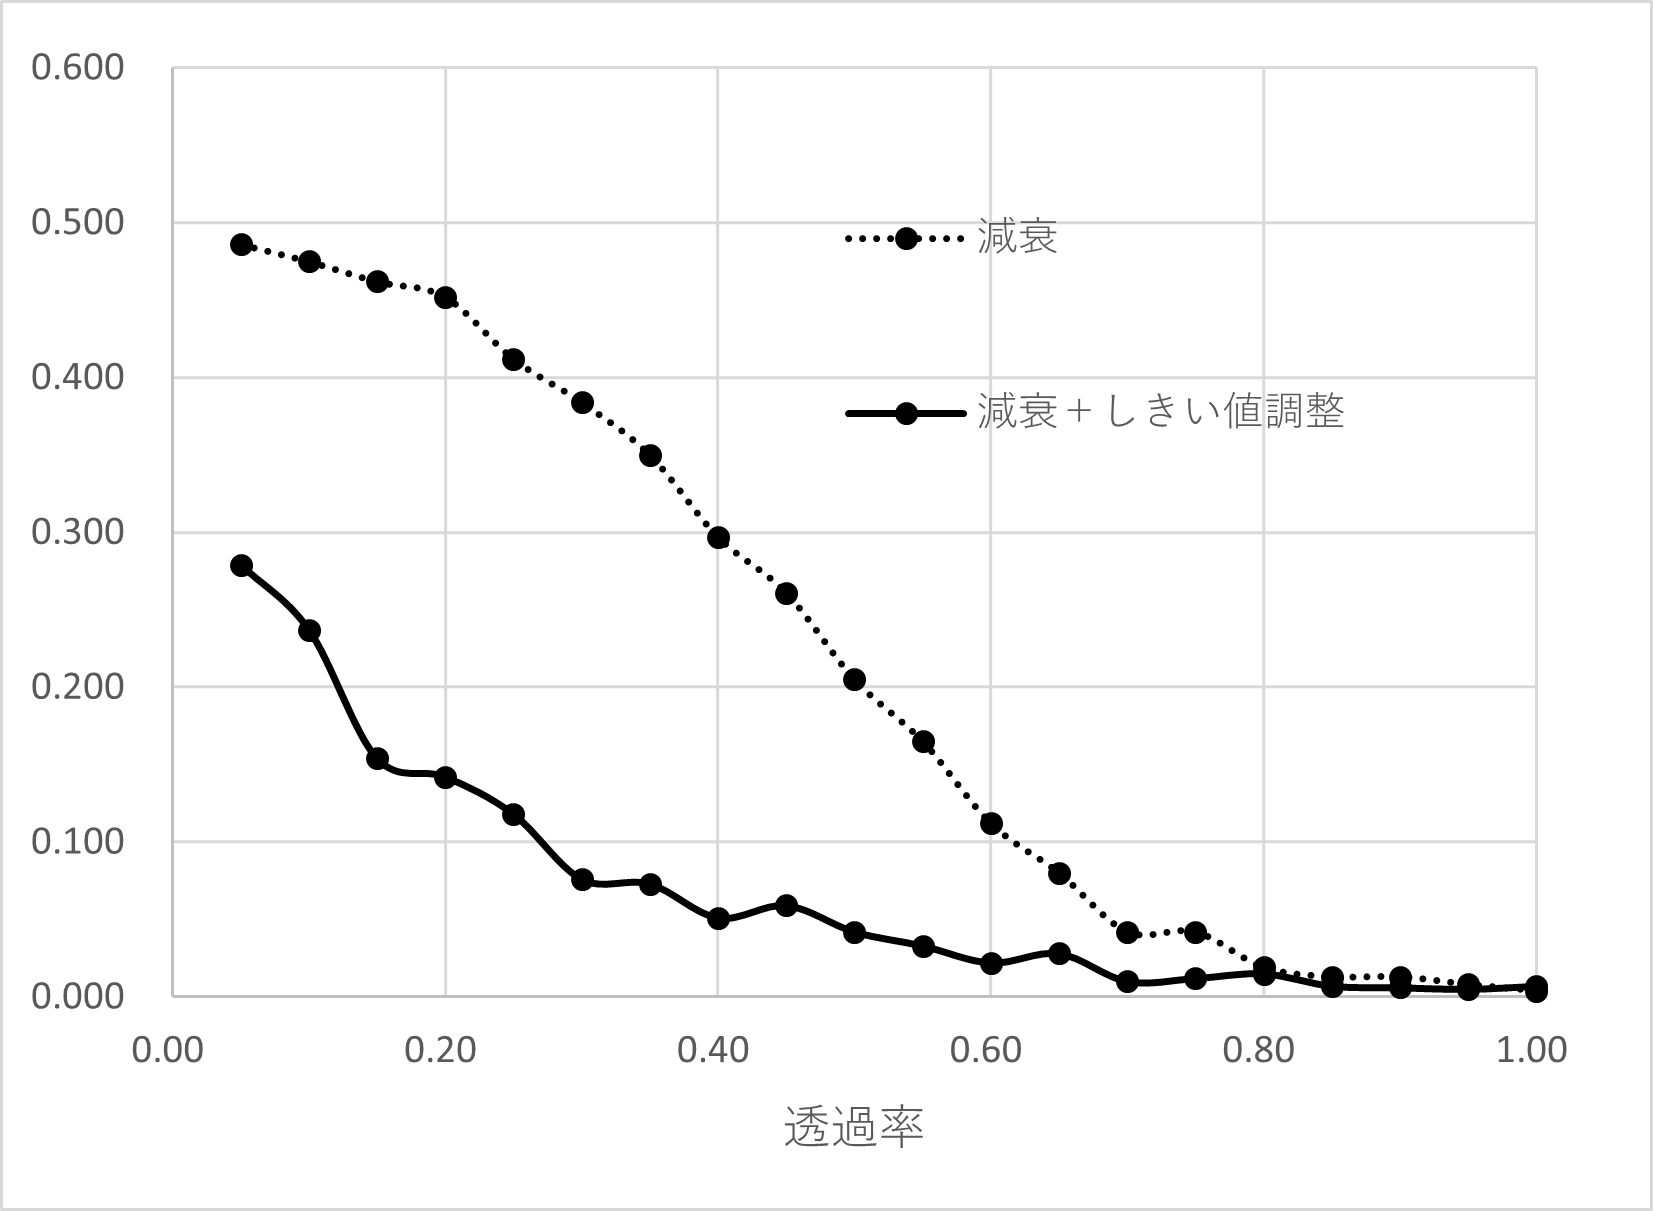
\includegraphics[width=0.4\textwidth]{img/zemi41.png}
        \caption[sample image (png)]{透過率と正規受信者の誤り率の関係.}
        \label{Fig:5_4}
    \end{figure}


次に,増幅器を減衰通信路の中間地点においた場合について考える.また,更に前置増幅を行った場合と前置増幅を行わずしきい値調整を行った場合の比較も合わせて行うことにする.\figref{Fig:5_5}は信号の最大強度が5,基底数が256,送信データ数が1000個の場合に透過率と正規受信者の誤り率の関係を表したものである.
\figref{Fig:5_5}により,前置増幅を行うことにより増幅のみを行った場合に比べて誤り率を下げることができることがわかる.ただし,増幅としきい値調整を行った場合に比べると誤り率は少し高くなっている.

\begin{figure}[htbp]
        \centering   
        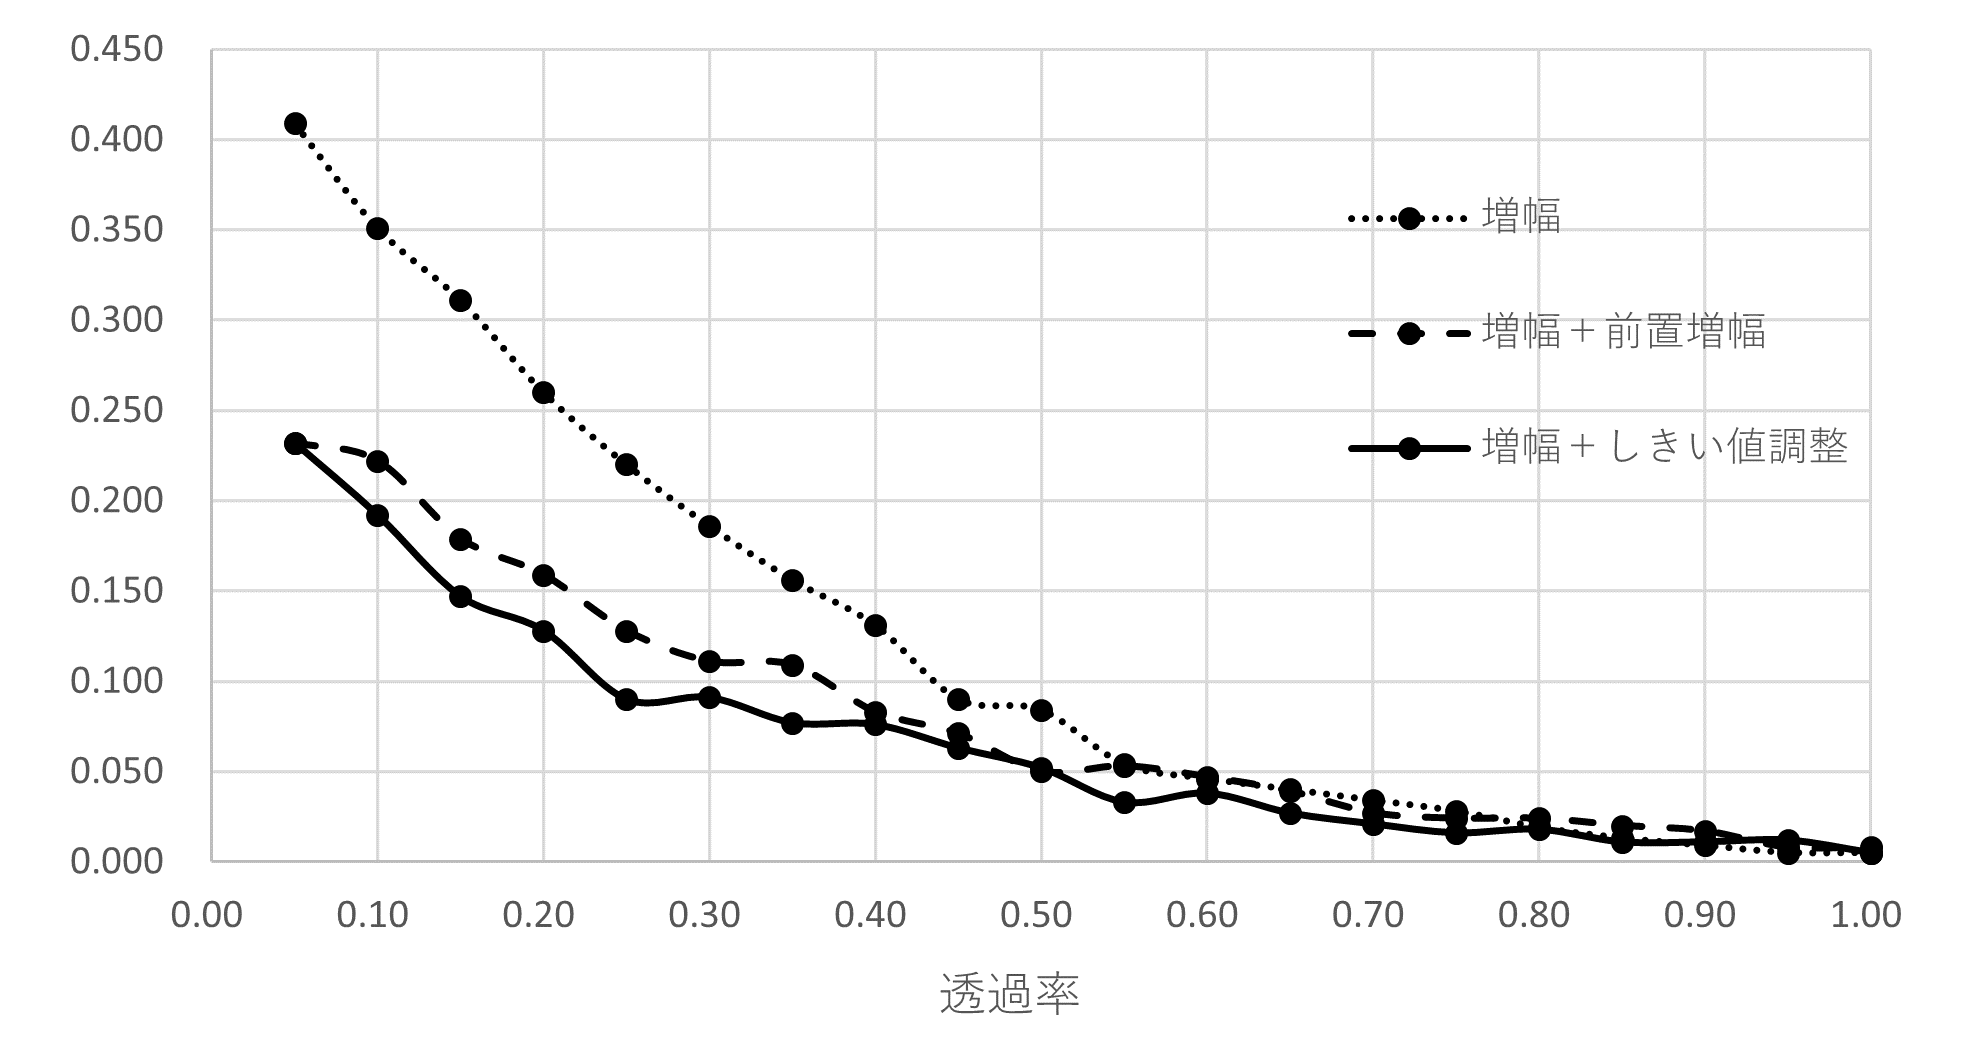
\includegraphics[width=0.5\textwidth]{img/zemi40.png}
        \caption[sample image (png)]{増幅の効果}
        \label{Fig:5_5}
    \end{figure}
    



\section{まとめ}
本研究ではY00-量子暗号のシミュレーションシステムを用いて正規受信者の誤り率の評価を行った.その結果,通信路の中間地点に増幅器を設置し,減衰に合わせて受信器でしきい値調整を行うことの有効性が確かめられた.



\begin{thebibliography}{9}
\bibitem{Futami}Fumio Futami and Osamu Hirota,Two Months Field
Transmission Test of 2.5-Gb/s Y-00 Cipher in 160-km (40 km x 4
spans)Installed Optical Fiber Cable for Secure Optical Fiber Communications,Tamagawa University Quantum ICT Research Institute Bulletin, Vol.2, No.1, 15-17, 2012 

\bibitem{久保}久保貴星,光通信量子暗号のシミュレーション, 玉川大学工学部情報通信工学科卒業論文,
\bibitem{井上}
井上恭,工学系のための量子工学,森北出版株式会社,2020 
\end{thebibliography}
\end{document}
